\section{Grundlagen}
\label{sec:fundamentals}

Das ist ein Bild, um zu sehen wie man es einbindet.
\begin{figure}[H]
\centering
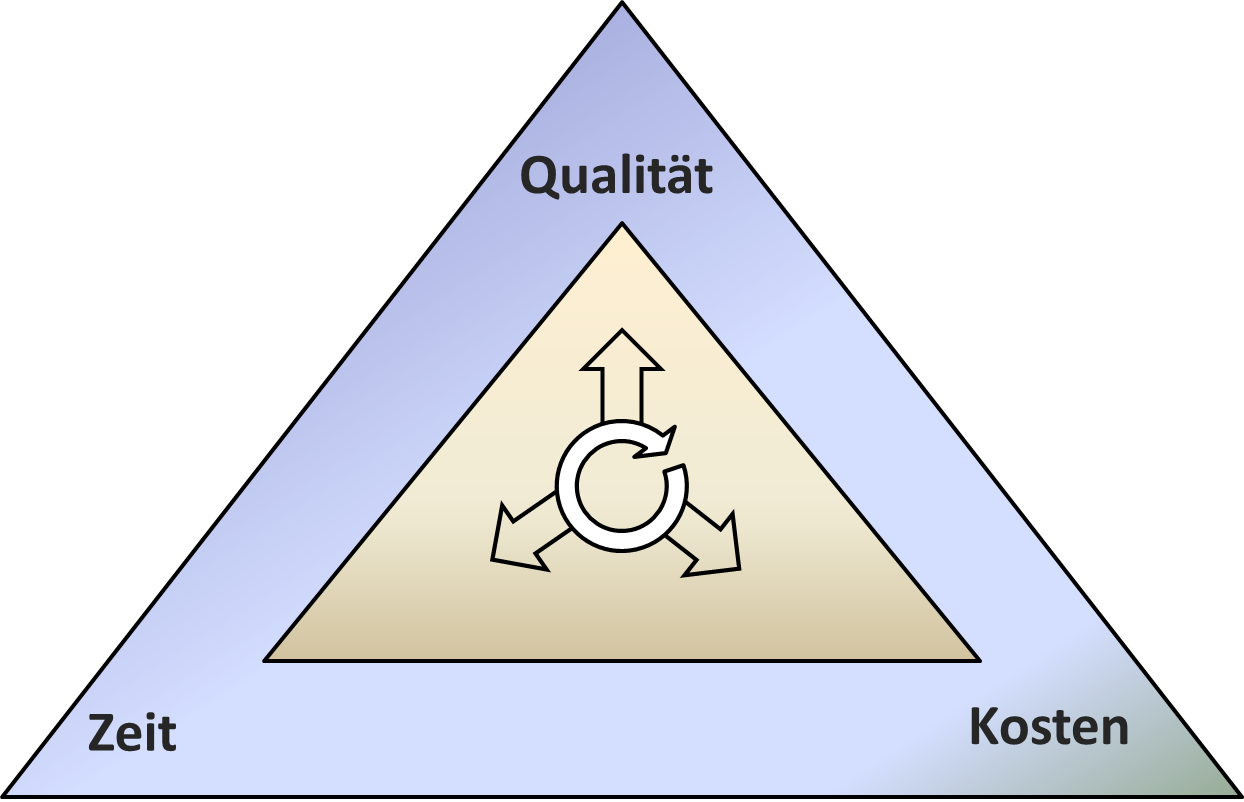
\includegraphics[width=1.1\textwidth]{../images/software_quality_triangle.PNG}
\caption[Software-Qualitätspyramide]{Software-Qualitätspyramide}
\label{fig:software_quality_triangle}
\end{figure}

Beispiel für eine Tabelle

\begin{table}[H]
\centering
\begin{tabular}{|l|p{9cm}|}
\hline
\rowcolor[HTML]{EFEFEF} 
\textit{\textbf{Qualitätsmerkmal}} & \textit{\textbf{Erläuterung}}       \\ \hline
\textbf{Änderbarkeit}              & Aufwand, der zur Durchführung vorgegebener Änderungen notwendig ist. Dies beinhaltet die Unterkategorien Änderungen, Analysierbarkeit, Modifizierbarkeit, Stabilität und Prüfbarkeit.
\\ \hline
\textbf{Benutzbarkeit}             &                                                                                                                                                                                                 Aufwand, den ein Benutzer der Software für das Verstehen und die Verwendung der Software aufbringen muss. Dieser beinhaltet die Unterkategorien Verständlichkeit, Erlernbarkeit und Bedienbarkeit.
 \\ \hline
\textbf{Effizienz}                 &                                                                                                                                                                                                    
Misst die Leistung der Software anhand des Zeitbedarfes, bei dessen Ausführen oder deren Ressourcenverbrauch.
\\ \hline
\textbf{Zuverlässigkeit}           &                                                                                                                                                                                                    
Eigenschaften, die ausdrücken, wie fehlertolerant eine Software ist, also wie intelligent auf Fehler reagiert wird.
\\ \hline
\textbf{Funktionalität}            &                                                                                                                                                                                                    
Die Übereinstimmung der Software mit der Spezifikation. Sie ist eine der wichtigsten Qualitätsmerkmale von Software, das ist die grundlegenden Eigenschaften zu den Funktionen der Software, was sie funktional leisten soll und wie. Darunter fallen, Richtigkeit, Angemessenheit, Ordnungsmäßigkeit, Interoperabilität und Sicherheit.
\\ \hline
\textbf{Übertragbarkeit}           &                                                                                                                                                                                                    
Sagt aus, ob eine Software auf unterschiedlichen Betriebssystemen mit verschiedener Hardwareausstattung ausgeführt werden kann.
\\ \hline
\end{tabular}
\caption{Qualitätsmerkmale und ihre Bedeutung für das Software-Produkt}
\label{quality_of_sortware}
\end{table}
Beispiel für eine Box mit Text

\fbox{\parbox{\columnwidth}{
Als Käufer möchte ich einen Artikel in meinen Warenkorb legen, damit ich diesen anschließend kaufen kann.
}}
